\documentclass[article,12pt,onesidea,4paper,english,brazil]{abntex2}

\usepackage{lmodern, indentfirst, nomencl, color, graphicx, microtype, lipsum}			
\usepackage[T1]{fontenc}		
\usepackage[utf8]{inputenc}		

\setlrmarginsandblock{2cm}{2cm}{*}
\setulmarginsandblock{2cm}{2cm}{*}
\checkandfixthelayout

\setlength{\parindent}{1.3cm}
\setlength{\parskip}{0.2cm}

\SingleSpacing

\begin{document}
	
	\selectlanguage{brazil}
	
	\frenchspacing 
	
	\begin{center}
		\LARGE 
		NOVAS TECNOLOGIAS PARA O ENSINO DE BIOLOGIA: A HISTOLOGIA NA REDE
		
		
		\normalsize
		Luciano Vieira Pereira\footnote{Bolsista PIBITI - CNPq, pereiralucianovieira@gmail.com, Campus Ariquemes.} 
		Bárbara Severo Jacob\footnote{Bolsista PIBITI - IFRO, barbara.jacobb@gmail.com, Campus Ariquemes} 
		Estéfane Oliveira de Moraes\footnote{Bolsista PIBIC EM – CNPq / IFRO, esteffmoraes@gmail.com, Campus Porto Velho Calama.} \\
	Jardson Yudi Ikenohuchi \footnote{Bolsista PIBIC EM – CNPq / IFRO, jardsonyudi@gmail.com, Campus Porto Velho Calama..} 
			Giselle Cavalcante Saldanha\footnote{Orientadora, giselle.andrade@ifro.edu.br, Campus Ariquemes}\\
				Willians de Paula Pereira\footnote{Co-orientador, willians.pereira@ifro.edu.br, Campus Porto Velho Calama}
				Elisangela Bibá Gomes Pinho\footnote{Co-orientadora, elisangela.pinho@ifro.edu.br, Campus Porto Velho Calama.}
	\end{center}
	
	% resumo em português
	\begin{resumoumacoluna}
	A necessidade de se adequar a velocidade com que as informações chegam aos alunos requer hoje professores atualizados e dinâmicos. O ensino da Histologia é realizado a partir da obtenção de informação visual, utilizando imagens microscópicas para posterior entendimento da função as células tecidos, órgãos e das transformações e processos a que estes estão sujeitos. O objetivo desta pesquisa consistiu de utilizar inovações metodológicas e tecnológicas como ferramentas de ensino/aprendizagem. No decorrer do projeto foram produzidos os um atlas virtual além de aulas, resumos e exercícios de fixação com linguagem e conteúdo apropriados para o ensino médio e que serão disponibilizados em um Espaço virtual como forma de auxílio no processo de ensino/aprendizagem.
		
		\vspace{\onelineskip}
		
		\noindent
		\textbf{Palavras-chave}:Formação de Professores. Aprendizagem. Tecnologia Educacional.
	\end{resumoumacoluna}
	
	\section*{Introdução}
	
	As necessidades de aulas mais dinâmicas usadas no em ensino de Biologia têm ressaltado a importância da utilização de metodologias inovadoras para contribuir no processo ensino/aprendizagem. Deste modo, destacamos a relevância dos estudos acerca da aprendizagem dos conceitos científicos, que ainda têm sido um grande desafio entre pesquisadores e profissionais da educação. Para que as informações possam chegar até os alunos os professores nos dias atuais precisam se adequar às novas tecnologias, e para isso eles necessitam estar sempre atualizados e com aulas mais dinâmicas, para que assim o processo de ensino e aprendizagem seja alcançado.
	
	Os objetos educacionais mais relevantes no processo de ensino-aprendizagem são o desenvolvimento da iniciativa, da capacidade de decidir e da persistência transmitir o conhecimento aos alunos. Já o papel do professor, nessa estratégia, é o de orientar, auxiliar a resolver as dificuldades que forem surgindo no decorrer das aulas. Uma das superações, ou um cuidado importante ao se trabalhar metodologias alternativas é dosar a participação do professor e a participação de cada um dos alunos, garantindo que esses tenham independência e orientação (KRASILCHIK, 2008).
	
	\section*{Material e Método}
	
	A execução do projeto de pesquisa foi dividida em duas etapas: elaboração do conteúdo referente à temática de histologia animal e desenvolvimento do espaço virtual para futura disponibilização do conteúdoproduzido.
	
	Todas as etapas relacionadas às atividades práticas do projeto foram realizadas no Instituto Federal de Educação, Ciência e Tecnologia – Campus Ariquemes-RO, no laboratório deBiologia.
	
	Para elaboração do conteúdo prático, ou seja, elaboração do mini atlas virtual, utilizou-se microscópio óptico convencional para observação de algumas estruturas dos tecidos nas lâminas que posteriormente foram analisadas no microscópio com tela de LCD. Para a elaboração do conteúdo teórico foram analisados os planos de curso e ensino anual de biologia, tanto do ensino médio e superior de biologia do Instituto Federal de Rondônia – Campus Ariquemes. Para que assim ocorressem às bases de consultas foram às obras de Gartner e Hiatt (1999) e Junqueira e Carneiro (2011). Nesta fase foram elaborados textos referentes a cada um dos tecidos estudados.
	
	O Espaço Virtual de Aprendizagem foi desenvolvido por meio de ferramentas de Software Livre que não necessitam da aquisição de licenças e são seguros para a tarefa proposta. Para maior facilidade de acesso foi desenvolvido em plataforma web para que não houvesse uma grande dificuldade em download e instalação do software,queinviabilizariaoacessofácilesimplesparaferramentaalternativade estudo. Para análise de técnica de sistema tudo foi baseado em diagramação e documentação UML.
	
	Para o desenvolvimento do software foram testadas as tecnologias Java por meio do framework Grails. Para desenvolvimento de software foi utilizada a linguagem de programação PHP, para ferramenta de desenvolvimento foi utilizado o XAMPP, pois possui pacote de código aberto atendendo os requisitos estabelecidos para melhor disponibilidade de conteúdos e manutenção. Para banco de dados utilizou-se PostegreSQL pois tem capacidade de crescer muito e muito em volume de dados sem deteriorar performance, ou crescer muito em termos de complexidade ou uso de mais módulos.
	
	
	
	\section*{Resultados e Discussão}
	
Foram produzidos materiais de cunho didático para posterior disponibilização no espaço virtual. A produção dos materiais foi realizada com foco no aprendizado de alunos do ensino médio, mas permitiu aos alunos da graduação, participantes da pesquisa, o aprofundamento de conhecimentos específicos de Biologia e propiciaram a construção e consolidação desses conhecimentos de maneira a promover o desenvolvimento da crítica e inovação nos processos pedagógicos.

Sabemos que aula de laboratório é ideal, porém é difícil de acontecer, pois depende de muitas pessoas (professor e alunos) e elas têm que estar motivadas (professor animado para aplicação das atividades e os alunos com vontade de aprender). Além da motivação, as aulas de laboratório inicialmente necessitam de preparo das atividades, e por fim material adequado disponível para estudo por parte da instituição. Pensando nisso um atlas histológico virtual, contendo 31( trinta e  uma) lâminas devidamente descritas e disponibilizadas em três tipos de aumento será disponibilizado aos usuários do espaço virtual. Dessa forma esta pesquisa poderá contribuir com o processo de ensino/aprendizagem entre professores e alunos envolvidos com a histologia animal, e que talvez não tenham recursos para a aula de laboratório.

O espaço virtual foi desenvolvido os protótipos planejados estão apresentados de acordo com as figuras 1e 2.

\begin{figure}[h]
	\centering
	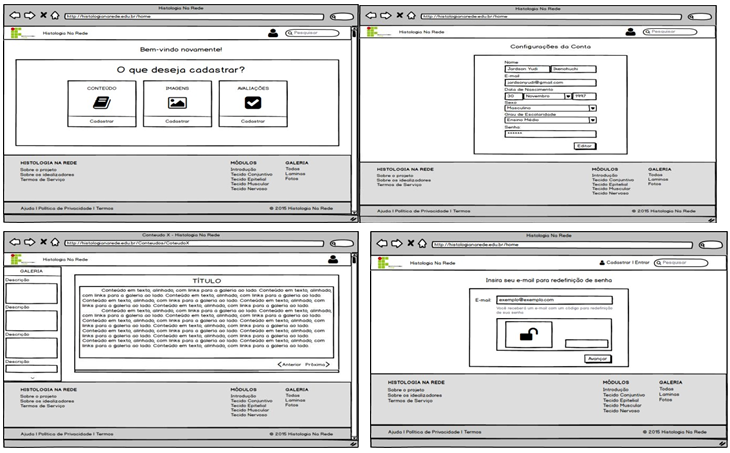
\includegraphics[width=0.6\linewidth]{pip-artigo12-01}
	\caption{Exemplos de protótipos planejados ao longo do desenvolvimento do trabalho – Da esquerda para direita: Página de Boas Vindas / Configurações da Conta / Módulos / Cadastro.}
	\label{fig:pip-artigo12-01}
\end{figure}
\begin{figure}[h]
	\centering
	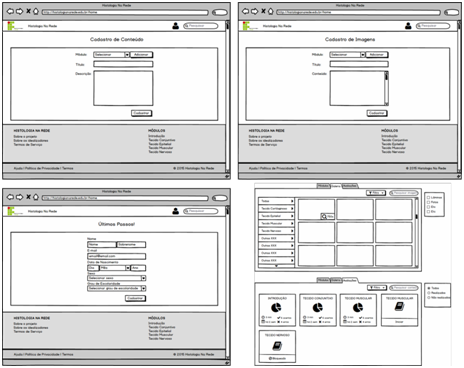
\includegraphics[width=0.6\linewidth]{pip-artigo12-02}
	\caption{Exemplos de protótipos planejados ao longo do desenvolvimento do trabalho – Da esquerda para direita: Cadastro de Conteúdos / Cadastro de Imagens / Últimos Passos/ Galeria.}
	\label{fig:pip-artigo12-02}
\end{figure}

Numa segunda fase da pesquisa o projeto será submetido à análise de Comitê de Ética para que o espaço virtual possa ser testado e avaliado por professores e estudantes da rede pública deensino.

	
	\section*{Conclusões}
	
Durante o desenvolvimento desta pesquisa foi possível promover a interação entre os graduandos em Ciências Biológicas e os alunos de Ensino Médio o que contribuiu para a formação reflexiva de futuros professores de Biologia que trabalharão nas escolas do estado de Rondônia.

Os resultados dessa pesquisa poderão contribuir, tanto com alunos e professores, pois o espaço virtual produzido poderá ser utilizado uma ferramenta que facilitará o processo de ensino eaprendizagem.
	
	\section*{Instituição de Fomento}
	
	CNPq e Pró-Reitoria de Pesquisa, Inovação e Pós-Graduação do IFRO.
	
	\section*{Referências}
	
\noindent KRASILCHIK, M. Prática de Ensino de Biologia. 6.ed. São Paulo: Edusp, 2008. JUNQUEIRA, L. C.; CARNEIRO, J. Histologia Básica. 11 ed. Rio de Janeiro: Guanabara Koogan, 2012.

\noindent SOBOTTA J. \& WELSCH U. SOBOTTA Atlas de Histologia – Citologia, Histologia e Anatomia Microscópica – 7ª Edição Editora Guanabara Koogan (Grupo GEN).2007.

\noindent GARTNER, L. P. \& Hiatt, J. L. Tratado de Histologia em Cores. 2 ed. Rio de Janeiro: Guanabara Koogan, 2003.
	
\end{document}